\chapter{Reaksi Kimia: Pereaksi dan Produk}\label{ch:g7:chemical-reactions}

Arang berpijar di pemanggang sate. Sejam kemudian hampir tidak ada yang
tersisa dari bongkahan-bongkahan hitam itu --- sedikit abu kelabu, dan
panas yang tadi memasak makanan. Ke mana perginya karbon yang hitam itu?
Karbon itu tidak lenyap: ia bertemu oksigen dari \omterm{def:g4:air-a-mixture-of-gases:air}{udara} dan menjadi gas
baru yang tidak terlihat. Dengan \omterm{def:g7:atoms-and-molecules:atom}{atom} dan \omterm{def:g7:atoms-and-molecules:molecule}{molekul} di tangan, kini kita
dapat mengatakan dengan tepat apa yang terjadi dalam perubahan seperti
itu.

\begin{recall}
Pada \omterm{def:g5:irreversible-changes:chemical-change}{perubahan kimia}, zat-zat baru muncul dan tidak ada jalan kembali
yang sederhana (\cref{ch:g5:irreversible-changes}). Air kapur menjadi
keruh oleh karbon dioksida, tembaga sulfat anhidrat menjadi biru oleh
air (\cref{ch:g7:identifying-substances}). Semua materi tersusun atas
\omterm{def:g7:atoms-and-molecules:atom}{atom}, yang berkelompok menjadi \omterm{def:g7:atoms-and-molecules:molecule}{molekul}; rumus seperti \ce{CO2}
mendaftar \omterm{def:g7:atoms-and-molecules:atom}{atom-atom} sebuah \omterm{def:g7:atoms-and-molecules:molecule}{molekul} (\cref{ch:g7:atoms-and-molecules}).
\end{recall}

\begin{omfigure}
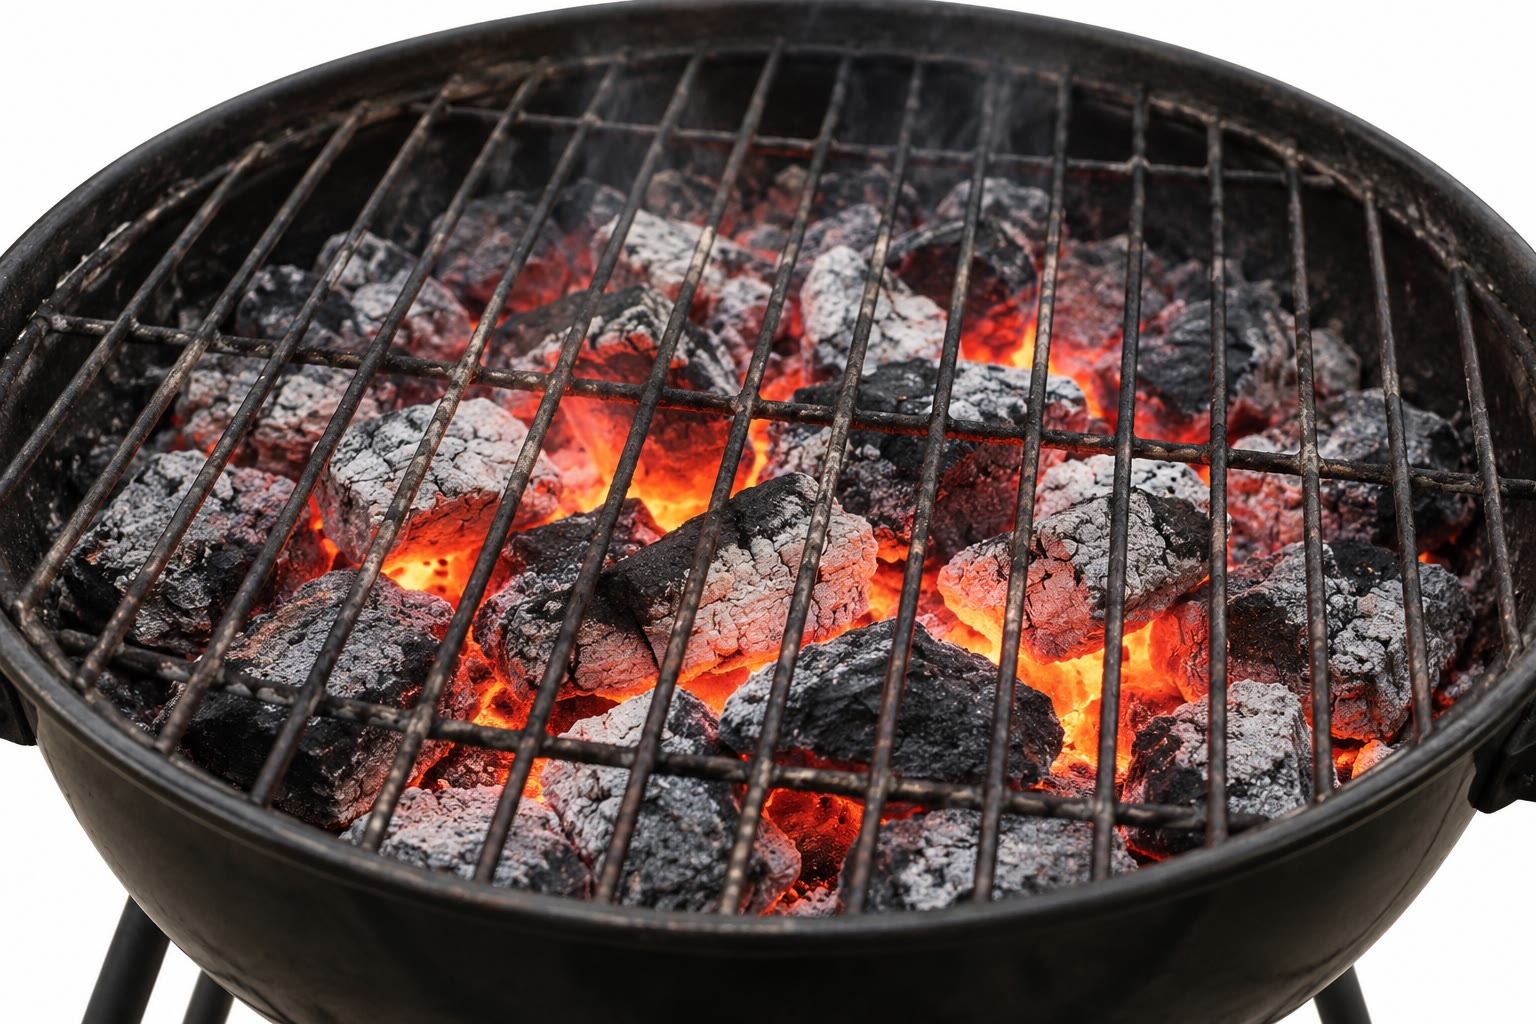
\includegraphics[width=0.55\linewidth]{images/book1/ai/g7-charcoal-bbq.jpg}

{\small Arang yang berpijar: karbon bereaksi dengan oksigen dari \omterm{def:g4:air-a-mixture-of-gases:air}{udara}.}
\end{omfigure}

\section{Perubahan fisika dan perubahan kimia}

\begin{definition}[Perubahan fisika]\label{def:g7:chemical-reactions:physical-transformation}
Sebuah \emph{perubahan fisika}\index{perubahan fisika} mengubah wujud
atau susunan materi tanpa mengubah \omterm{def:g6:pure-substances-and-mixtures:species}{spesies kimianya}: mencair, membeku,
mendidih, melarut, bercampur. Spesies yang sama ada sebelum dan
sesudahnya; hanya bentuk atau susunannya yang berubah.
\end{definition}

\begin{example}[Air, tiga cara]\label{ex:g7:chemical-reactions:water}
Es yang mencair menjadi air, air yang mendidih menjadi uap air, dan
garam yang \omterm{def:g2:mixing-and-dissolving:dissolve}{larut} dalam air adalah \omterm{def:g7:chemical-reactions:physical-transformation}{perubahan fisika}: sebelum dan
sesudahnya, ada \omterm{def:g7:atoms-and-molecules:molecule}{molekul} air (dan garam). Jika diperbesar, \omterm{def:g7:atoms-and-molecules:molecule}{molekulnya}
sama; hanya cara \omterm{def:g7:atoms-and-molecules:molecule}{molekul-molekul} itu tersusun dan bergerak yang berubah.
\end{example}

\begin{proposition}[Perubahan kimia]\label{prop:g7:chemical-reactions:chemical}
Pada \omterm{def:g5:irreversible-changes:chemical-change}{perubahan kimia}, sebagian \omterm{def:g6:pure-substances-and-mixtures:species}{spesies kimia} hilang dan spesies baru
muncul. \omterm{def:g5:irreversible-changes:chemical-change}{Perubahan kimia} dibedakan dari \omterm{def:g7:chemical-reactions:physical-transformation}{perubahan fisika} oleh
\omterm{def:g7:chemical-reactions:reactant}{produknya}: spesies-spesies baru, yang dapat dideteksi dengan \omterm{def:g7:identifying-substances:characteristic-test}{uji khas}.
\end{proposition}

\begin{omfigure}
\begin{tikzpicture}[font=\small, level distance=1.5cm,
    box/.style={draw=omDef, fill=omDef!6, rounded corners=2pt, align=center,
      inner sep=4pt},
    level 1/.style={sibling distance=6.6cm},
    edge from parent/.style={draw, thick, omDef, ->}]
  \node[box] {sebuah perubahan materi}
    child {node[box, text width=5.2cm] {\textbf{fisika}: spesies yang sama\\
      sebelum dan sesudahnya\\ \footnotesize mencair, mendidih, melarut, bercampur}}
    child {node[box, draw=omProp, fill=omProp!6, text width=5.2cm]
      {\textbf{kimia}: spesies hilang,\\ spesies baru muncul\\
      \footnotesize pembakaran, perkaratan, memasak}};
\end{tikzpicture}

{\small Dua jenis perubahan.}
\end{omfigure}

\section{Pereaksi dan produk}

\begin{definition}[Reaksi kimia]\label{def:g7:chemical-reactions:reaction}
Sebuah \emph{reaksi kimia}\index{reaksi kimia} adalah model yang dipakai
para ahli kimia untuk sebuah \omterm{def:g5:irreversible-changes:chemical-change}{perubahan kimia}: reaksi itu mendaftar
spesies yang terpakai dan spesies yang terbentuk.
\end{definition}

\begin{definition}[Pereaksi dan produk]\label{def:g7:chemical-reactions:reactant}
Spesies yang terpakai dalam sebuah \omterm{def:g7:chemical-reactions:reaction}{reaksi kimia} disebut
\emph{pereaksi}\index{pereaksi}; spesies yang terbentuk disebut
\emph{produk}\index{produk}.
\end{definition}

\begin{example}[Karbon terbakar dalam oksigen]\label{ex:g7:chemical-reactions:carbon}
Ketika arang \omterm{def:g4:what-a-fire-needs:burning}{terbakar}, \omterm{def:g7:chemical-reactions:reactant}{pereaksinya} adalah karbon (arang itu) dan oksigen
(dari \omterm{def:g4:air-a-mixture-of-gases:air}{udara}). \omterm{def:g7:chemical-reactions:reactant}{Produknya} adalah karbon dioksida: jika dikocok dengan air
kapur, gas yang tertinggal di dalam stoples mengeruhkannya.
\end{example}

\begin{inthelab}[Arang di dalam stoples oksigen]
Guru memanaskan sepotong kecil arang di atas sendok \omterm{def:g4:what-a-fire-needs:burning}{pembakaran} sampai
berpijar, lalu menurunkannya ke dalam stoples berisi oksigen. Arang itu
berpijar jauh lebih terang daripada di \omterm{def:g4:air-a-mixture-of-gases:air}{udara} dan menyusut sampai habis.
Stoples itu ditutup, sedikit air kapur dituangkan ke dalamnya lalu
dikocok: air kapur menjadi keruh. Karbon dan oksigen telah terpakai;
karbon dioksida telah terbentuk.
\end{inthelab}

\begin{omfigure}
\begin{tikzpicture}[font=\small, scale=1.3]
  \pic[transform shape] at (0,0) {gasjaropen={0}{white}};
  \fill[omWater!60] (-0.68,2.62) rectangle (0.68,2.7);
  \draw[omGlass, line width=0.4pt] (-0.68,2.62) rectangle (0.68,2.7);
  \draw[black!60, line width=1.2pt] (0.15,2.7) -- (0.15,3.6) -- (1.2,3.6);
  \draw[black!60, line width=1.2pt] (0.15,2.7) -- (0.15,1.2);
  \fill[black!60] (-0.12,1.12) rectangle (0.32,1.2);
  \fill[red!70!black] (0.0,1.32) circle (0.13);
  \fill[orange!90!yellow] (0.0,1.32) circle (0.08);
  \draw[<-, omProp, thick] (0.15,1.35) -- (1.5,1.6) node[right, text=black]
    {arang berpijar (karbon)};
  \draw[<-, omProp, thick] (-0.35,2.1) -- (1.5,2.3) node[right, text=black]
    {oksigen};
  \draw[<-, omProp, thick] (0.6,2.66) -- (1.5,2.95) node[right, text=black]
    {tutup};
  \draw[<-, omProp, thick] (0.15,3.1) -- (1.5,3.6) node[right, text=black]
    {sendok pembakaran};
\end{tikzpicture}

{\small Arang berpijar yang diturunkan dengan sendok ke dalam stoples
oksigen menyala terang: karbon dan oksigen bereaksi membentuk karbon
dioksida.}
\end{omfigure}

\begin{example}[Wol baja]\label{ex:g7:chemical-reactions:steel-wool}
Segumpal wol baja halus, yang sebagian besar berupa besi, dapat \omterm{def:g4:what-a-fire-needs:burning}{terbakar}
di \omterm{def:g4:air-a-mixture-of-gases:air}{udara} dengan hamburan bunga api. \omterm{def:g7:chemical-reactions:reactant}{Pereaksinya} adalah besi dan oksigen;
\omterm{def:g7:chemical-reactions:reactant}{produknya} adalah padatan gelap yang mudah remuk, sebuah oksida besi.
\end{example}

\begin{omfigure}
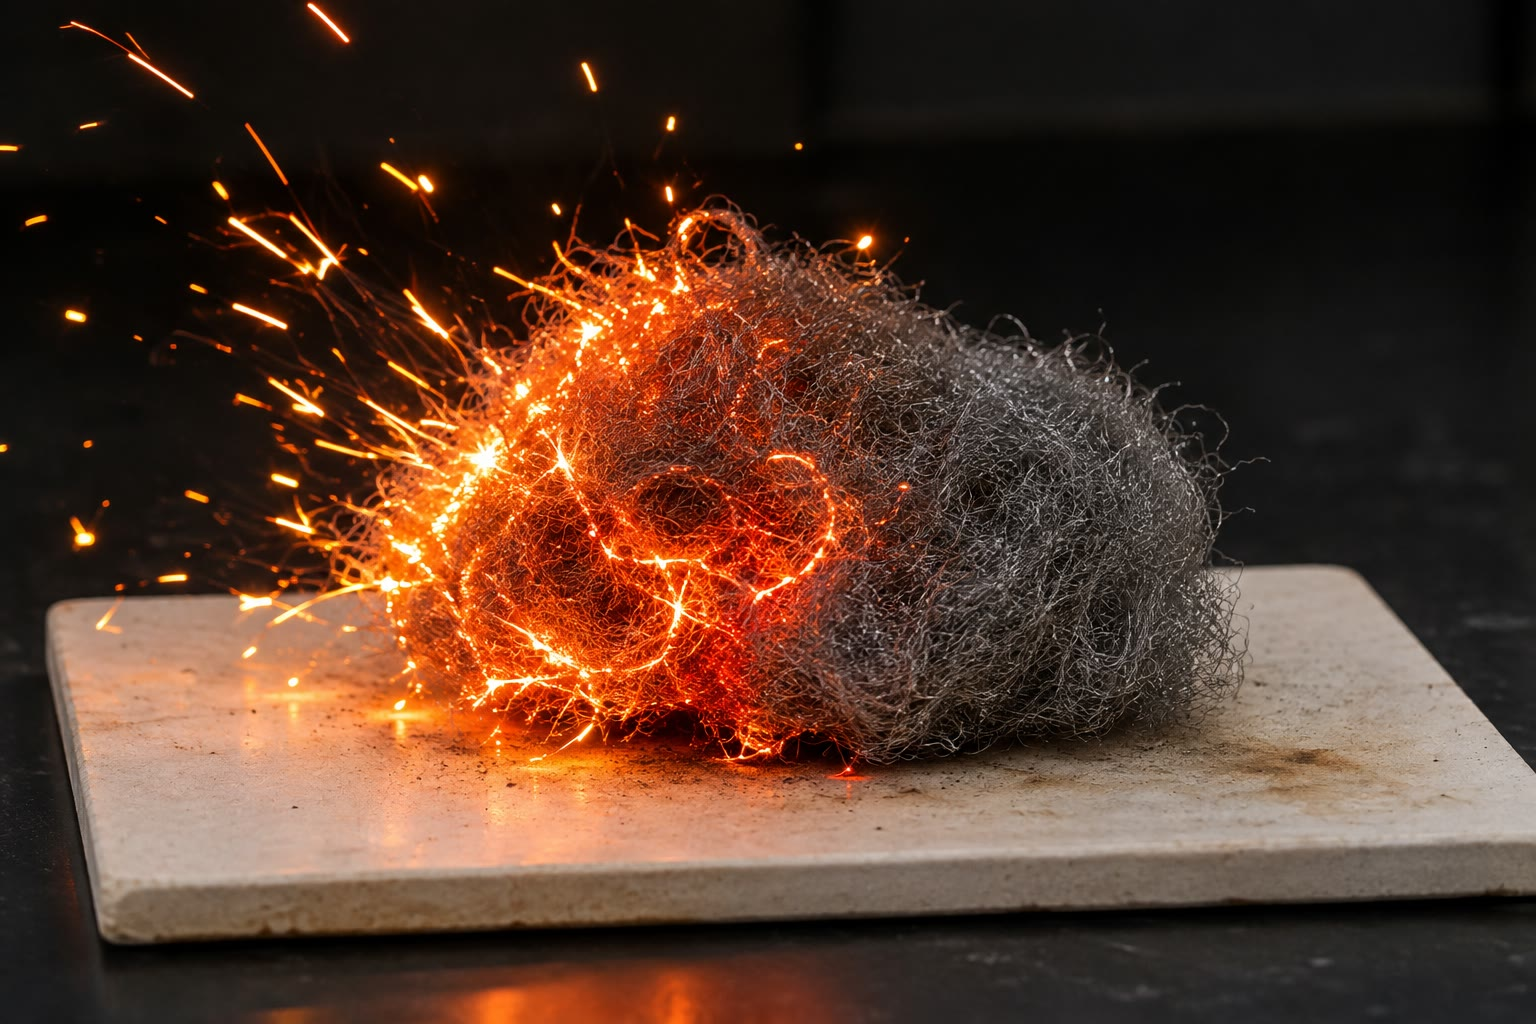
\includegraphics[width=0.5\linewidth]{images/book1/ai/g7-steel-wool-burning.jpg}

{\small Wol baja \omterm{def:g4:what-a-fire-needs:burning}{terbakar} di laboratorium: besi dan oksigen bereaksi.}
\end{omfigure}

\section{Persamaan kata}

\begin{definition}[Persamaan kata]\label{def:g7:chemical-reactions:word-equation}
Sebuah \emph{persamaan kata}\index{persamaan kata} menuliskan \omterm{def:g7:chemical-reactions:reaction}{reaksi
kimia} dengan kata-kata: nama-nama \omterm{def:g7:chemical-reactions:reactant}{pereaksi} di kiri, dihubungkan dengan
$+$, sebuah anak panah, dan nama-nama \omterm{def:g7:chemical-reactions:reactant}{produk} di kanan. Anak panah itu
dibaca ``bereaksi menghasilkan''.
\end{definition}

\begin{example}[Tiga persamaan kata]\label{ex:g7:chemical-reactions:three}
\begin{center}
\begin{tabular}{l}
karbon $+$ oksigen $\longrightarrow$ karbon dioksida\\[2pt]
metana $+$ oksigen $\longrightarrow$ karbon dioksida $+$ air\\[2pt]
besi $+$ oksigen $\longrightarrow$ oksida besi
\end{tabular}
\end{center}
\end{example}

\begin{method}[Menuliskan persamaan kata]\label{met:g7:chemical-reactions:write}
\begin{enumerate}
  \item Tentukan \omterm{def:g7:chemical-reactions:reactant}{pereaksinya}: spesies yang hilang.
  \item Tentukan \omterm{def:g7:chemical-reactions:reactant}{produknya}: spesies baru, yang dikenali dengan uji.
  \item Tuliskan \omterm{def:g7:chemical-reactions:reactant}{pereaksi} di kiri, \omterm{def:g7:chemical-reactions:reactant}{produk} di kanan, dengan anak panah di
        antaranya; jangan pernah tanda sama dengan.
\end{enumerate}
Spesies yang ada tetapi tidak ikut bereaksi --- nitrogen di \omterm{def:g4:air-a-mixture-of-gases:air}{udara} di
sekitar nyala api --- tidak dituliskan.
\end{method}

\section{Reaksi adalah penataan ulang atom}

\begin{proposition}[Atom-atom ditata ulang]\label{prop:g7:chemical-reactions:rearranged}
Dalam \omterm{def:g7:chemical-reactions:reaction}{reaksi kimia}, \omterm{def:g7:atoms-and-molecules:molecule}{molekul-molekul} \omterm{def:g7:chemical-reactions:reactant}{pereaksi} terurai dan \omterm{def:g7:atoms-and-molecules:atom}{atom-atomnya}
bergabung dengan cara lain untuk membangun \omterm{def:g7:atoms-and-molecules:molecule}{molekul-molekul} \omterm{def:g7:chemical-reactions:reactant}{produk}.
\omterm{def:g7:atoms-and-molecules:atom}{Atom-atom} itu sendiri tidak diciptakan dan tidak dimusnahkan: \omterm{def:g7:atoms-and-molecules:atom}{atom-atom}
yang sama, dalam jumlah yang sama, ada sebelum dan sesudahnya.
\end{proposition}

\begin{example}[Metana terbakar, molekul demi molekul]\label{ex:g7:chemical-reactions:methane}
Ketika metana dari kompor gas \omterm{def:g4:what-a-fire-needs:burning}{terbakar}, satu \omterm{def:g7:atoms-and-molecules:molecule}{molekul} metana \ce{CH4}
bertemu dua \omterm{def:g7:atoms-and-molecules:molecule}{molekul} oksigen \ce{O2}. \omterm{def:g7:atoms-and-molecules:atom}{Atom-atomnya} tertata ulang menjadi
satu \omterm{def:g7:atoms-and-molecules:molecule}{molekul} karbon dioksida \ce{CO2} dan dua \omterm{def:g7:atoms-and-molecules:molecule}{molekul} air \ce{H2O}.
Sebelum: 1 \omterm{def:g7:atoms-and-molecules:atom}{atom} karbon, 4 hidrogen, dan 4 oksigen. Sesudah: 1 karbon, 4
hidrogen, dan $2 + 2 = 4$ \omterm{def:g7:atoms-and-molecules:atom}{atom} oksigen. Tidak ada yang hilang, tidak ada
yang muncul entah dari mana.
\end{example}

\begin{omfigure}
\begin{tikzpicture}[font=\small]
  % methane
  \begin{scope}[xshift=0cm]
    \node[aC] (c) at (0,0) {};
    \node[aH] (h1) at (0,0.78) {}; \node[aH] (h2) at (-0.74,-0.3) {};
    \node[aH] (h3) at (0.74,-0.3) {}; \node[aH] (h4) at (0.2,-0.68) {};
    \begin{scope}[on background layer]
      \foreach \h in {h1,h2,h3,h4} \draw[bond] (c.center) -- (\h.center);
    \end{scope}
    \node at (0,-1.2) {1 metana};
  \end{scope}
  \node at (1.45,0) {$+$};
  % two oxygen molecules
  \foreach \y in {0.45,-0.45} {
    \node[aO] (a) at (2.4,\y) {}; \node[aO] (b) at (3.05,\y) {};
    \begin{scope}[on background layer]
      \draw[bond, line width=1.1pt] ([yshift=1.6pt]a.center) -- ([yshift=1.6pt]b.center);
      \draw[bond, line width=1.1pt] ([yshift=-1.6pt]a.center) -- ([yshift=-1.6pt]b.center);
    \end{scope}
  }
  \node at (2.72,-1.2) {2 oksigen};
  \draw[->, thick, omProp] (3.8,0) -- (5.0,0);
  % carbon dioxide
  \begin{scope}[xshift=6.3cm]
    \node[aO] (a) at (-0.8,0) {}; \node[aC] (c) at (0,0) {}; \node[aO] (b) at (0.8,0) {};
    \begin{scope}[on background layer]
      \foreach \d in {-1.6,1.6} {
        \draw[bond, line width=1.1pt] ([yshift=\d pt]a.center) -- ([yshift=\d pt]c.center);
        \draw[bond, line width=1.1pt] ([yshift=\d pt]c.center) -- ([yshift=\d pt]b.center);}
    \end{scope}
    \node at (0,-1.2) {1 karbon dioksida};
  \end{scope}
  \node at (7.8,0) {$+$};
  % two water molecules
  \foreach \x in {8.9,10.6} {
    \node[aO] (o) at (\x,0.2) {};
    \node[aH] (p) at (\x-0.58,-0.25) {}; \node[aH] (q) at (\x+0.58,-0.25) {};
    \begin{scope}[on background layer]
      \draw[bond] (o.center) -- (p.center); \draw[bond] (o.center) -- (q.center);
    \end{scope}
  }
  \node at (9.75,-1.2) {2 air};
  % atom counts
  \node[align=center, font=\footnotesize] at (1.5,-2.0) {sebelum: 1 C, 4 H, 4 O};
  \node[align=center, font=\footnotesize] at (8.5,-2.0) {sesudah: 1 C, 4 H, 4 O};
\end{tikzpicture}

{\small \omterm{def:g4:what-a-fire-needs:burning}{Pembakaran} metana, digambar dengan model \omterm{def:g7:atoms-and-molecules:molecule}{molekul}: \omterm{def:g7:atoms-and-molecules:atom}{atom-atom}
\omterm{def:g7:chemical-reactions:reactant}{pereaksi} tertata ulang menjadi \omterm{def:g7:chemical-reactions:reactant}{produk}. \omterm{def:g7:atoms-and-molecules:atom}{Atom-atom} yang sama dihitung
sebelum dan sesudahnya.}
\end{omfigure}

\begin{remark}[Menghitung molekul]\label{rem:g7:chemical-reactions:counting}
\omterm{def:g7:chemical-reactions:word-equation}{Persamaan kata} tidak mengatakan berapa \omterm{def:g7:atoms-and-molecules:molecule}{molekul} yang bereaksi: untuk itu,
persamaannya ditulis dengan rumus dan angka di depannya. Menuliskan
persamaan seperti itu, dan menemukan angka-angka yang tepat, menjadi
pokok bahasan sebuah bab berikutnya.
\end{remark}

\section{Latihan}

\begin{exercise}[$\star$]\label{exo:g7:chemical-reactions:1}
\omterm{def:g7:chemical-reactions:physical-transformation}{Perubahan fisika} atau \omterm{def:g5:irreversible-changes:chemical-change}{perubahan kimia}? Es yang mencair, korek api yang
\omterm{def:g4:what-a-fire-needs:burning}{terbakar}, gula yang \omterm{def:g2:mixing-and-dissolving:dissolve}{larut}, roti yang dipanggang, paku yang berkarat.
\end{exercise}

\begin{exercise}[$\star$]\label{exo:g7:chemical-reactions:2}
Apa yang dimaksud dengan \omterm{def:g7:chemical-reactions:reactant}{pereaksi} dan \omterm{def:g7:chemical-reactions:reactant}{produk} sebuah \omterm{def:g7:chemical-reactions:reaction}{reaksi kimia}?
\end{exercise}

\begin{exercise}[$\star$]\label{exo:g7:chemical-reactions:3}
Tuliskan \omterm{def:g7:chemical-reactions:word-equation}{persamaan kata} untuk \omterm{def:g4:what-a-fire-needs:burning}{pembakaran} karbon dalam oksigen.
\end{exercise}

\begin{exercise}[$\star$]\label{exo:g7:chemical-reactions:4}
Pada \omterm{def:g7:chemical-reactions:word-equation}{persamaan kata} ``besi $+$ oksigen $\longrightarrow$ oksida besi'',
sebutkan \omterm{def:g7:chemical-reactions:reactant}{pereaksi} dan \omterm{def:g7:chemical-reactions:reactant}{produknya}.
\end{exercise}

\begin{exercise}[$\star\star$]\label{exo:g7:chemical-reactions:5}
Ketika metana \omterm{def:g4:what-a-fire-needs:burning}{terbakar}, gelas dingin yang dipegang di atas nyalanya
berembun, dan gas yang ditampung mengeruhkan air kapur. \omterm{def:g7:chemical-reactions:reactant}{Produk} apa yang
ditunjukkan oleh kedua uji ini?
\end{exercise}

\begin{exercise}[$\star\star$]\label{exo:g7:chemical-reactions:6}
Seng bereaksi dengan asam klorida: sengnya hilang, gelembung hidrogen
dilepaskan, dan seng klorida tinggal di dalam larutan. Tuliskan
\omterm{def:g7:chemical-reactions:word-equation}{persamaan katanya}.
\end{exercise}

\begin{exercise}[$\star\star$]\label{exo:g7:chemical-reactions:7}
Lihatlah gambar model \omterm{def:g4:what-a-fire-needs:burning}{pembakaran} metana. Hitung \omterm{def:g7:atoms-and-molecules:atom}{atom} hidrogen sebelum
dan sesudah reaksi.
\end{exercise}

\begin{exercise}[$\star\star$]\label{exo:g7:chemical-reactions:8}
Mengapa melarutkan garam dalam air bukan \omterm{def:g7:chemical-reactions:reaction}{reaksi kimia}, meskipun garam
itu hilang dari pandangan?
\end{exercise}

\begin{exercise}[$\star\star$]\label{exo:g7:chemical-reactions:9}
Sebatang kayu gelondongan \omterm{def:g4:what-a-fire-needs:burning}{terbakar} habis menjadi setumpuk kecil abu.
Jelaskan, dengan memakai kata ``\omterm{def:g7:chemical-reactions:reactant}{produk}'', mengapa abunya jauh lebih
ringan daripada kayunya.
\end{exercise}

\begin{exercise}[$\star\star$]\label{exo:g7:chemical-reactions:10}
Hidrogen \omterm{def:g4:what-a-fire-needs:burning}{terbakar} dalam oksigen dan hanya menghasilkan air. Tuliskan
\omterm{def:g7:chemical-reactions:word-equation}{persamaan katanya}, dan sebutkan uji yang dapat mengenali \omterm{def:g7:chemical-reactions:reactant}{produknya}.
\end{exercise}

\begin{exercise}[$\star\star\star$]\label{exo:g7:chemical-reactions:11}
Dua \omterm{def:g7:atoms-and-molecules:molecule}{molekul} hidrogen \ce{H2} bereaksi dengan satu \omterm{def:g7:atoms-and-molecules:molecule}{molekul} oksigen
\ce{O2} menghasilkan dua \omterm{def:g7:atoms-and-molecules:molecule}{molekul} air \ce{H2O}. Hitung \omterm{def:g7:atoms-and-molecules:atom}{atom-atom} dari
setiap jenis sebelum dan sesudahnya, dan tunjukkan bahwa tidak ada yang
diciptakan atau dimusnahkan.
\end{exercise}

\begin{exercise}[$\star\star\star$]\label{exo:g7:chemical-reactions:12}
Seorang siswa menggambarkan \omterm{def:g4:what-a-fire-needs:burning}{pembakaran} karbon sebagai: satu \omterm{def:g7:atoms-and-molecules:atom}{atom} karbon
$+$ satu \omterm{def:g7:atoms-and-molecules:molecule}{molekul} oksigen $\longrightarrow$ satu \omterm{def:g7:atoms-and-molecules:molecule}{molekul} karbon dioksida
dan satu \omterm{def:g7:atoms-and-molecules:atom}{atom} oksigen yang tersisa. Apa yang salah dengan gambar ini?
Gambarkan yang benar dengan kata-kata.
\end{exercise}

\section{Soal: Di Dalam Nyala Kompor Gas}

\begin{problem}[{Soal akhir pekan --- apa yang terbakar dalam nyala kompor
gas, apa yang dihasilkannya, dan berapa molekul yang ikut serta}]
\label{pb:g7:chemical-reactions:1}
Gas pada kompor dapur sebagian besar berupa metana, \ce{CH4}. Dalam
nyalanya yang biru, metana bereaksi dengan oksigen dari \omterm{def:g4:air-a-mixture-of-gases:air}{udara}. Di
laboratorium, guru memegang sebuah gelas kimia yang dingin dan kering
secara terbalik di atas nyala seperti itu selama beberapa detik, lalu
membaliknya, menuangkan sedikit air kapur ke dalamnya, dan mengocoknya.

\medskip
\noindent\textbf{Bagian I --- \omterm{def:g7:chemical-reactions:reactant}{Pereaksi} dan \omterm{def:g7:chemical-reactions:reactant}{produk}.}
\begin{enumerate}
  \item Sebutkan kedua \omterm{def:g7:chemical-reactions:reactant}{pereaksi} reaksi ini.
  \item Titik-titik air muncul di dalam gelas kimia yang dingin; setetes
        darinya membirukan tembaga sulfat anhidrat. \omterm{def:g7:chemical-reactions:reactant}{Produk} apa yang
        ditunjukkan hal ini?
  \item Air kapurnya menjadi keruh. \omterm{def:g7:chemical-reactions:reactant}{Produk} lain apa yang ditunjukkan hal
        ini?
  \item \omterm{def:g4:air-a-mixture-of-gases:air}{Udara} juga mengandung nitrogen, yang melewati nyala api tanpa
        berubah. Apakah nitrogen sebuah \omterm{def:g7:chemical-reactions:reactant}{pereaksi}? Haruskah nitrogen
        muncul dalam \omterm{def:g7:chemical-reactions:word-equation}{persamaan kata}?
\end{enumerate}

\medskip
\noindent\textbf{Bagian II --- \omterm{def:g7:chemical-reactions:word-equation}{Persamaan kata}.}
\begin{enumerate}[resume]
  \item Tuliskan \omterm{def:g7:chemical-reactions:word-equation}{persamaan kata} reaksi itu.
  \item Apakah \omterm{def:g4:what-a-fire-needs:burning}{pembakaran} metana sebuah \omterm{def:g7:chemical-reactions:physical-transformation}{perubahan fisika} atau \omterm{def:g5:irreversible-changes:chemical-change}{perubahan
        kimia}? Berikan dua alasan.
  \item Tuliskan rumus keempat spesies dalam reaksi itu.
\end{enumerate}

\medskip
\noindent\textbf{Bagian III --- Menghitung \omterm{def:g7:atoms-and-molecules:molecule}{molekul}.}
Setiap \omterm{def:g7:atoms-and-molecules:molecule}{molekul} metana yang \omterm{def:g4:what-a-fire-needs:burning}{terbakar} bereaksi dengan dua \omterm{def:g7:atoms-and-molecules:molecule}{molekul} oksigen,
dan menghasilkan satu \omterm{def:g7:atoms-and-molecules:molecule}{molekul} karbon dioksida dan dua \omterm{def:g7:atoms-and-molecules:molecule}{molekul} air.
\begin{enumerate}[resume]
  \item Hitung \omterm{def:g7:atoms-and-molecules:atom}{atom} karbon, hidrogen, dan oksigen dalam satu \omterm{def:g7:atoms-and-molecules:molecule}{molekul}
        metana dan dua \omterm{def:g7:atoms-and-molecules:molecule}{molekul} oksigen, bersama-sama.
  \item Hitung \omterm{def:g7:atoms-and-molecules:atom}{atom-atom} itu dalam satu \omterm{def:g7:atoms-and-molecules:molecule}{molekul} karbon dioksida dan dua
        \omterm{def:g7:atoms-and-molecules:molecule}{molekul} air, bersama-sama. Apa yang kamu perhatikan?
  \item Nyala itu membakar 10 \omterm{def:g7:atoms-and-molecules:molecule}{molekul} metana. Berapa \omterm{def:g7:atoms-and-molecules:molecule}{molekul} oksigen
        yang dipakainya?
  \item Berapa \omterm{def:g7:atoms-and-molecules:molecule}{molekul} karbon dioksida yang dihasilkannya?
  \item Berapa \omterm{def:g7:atoms-and-molecules:molecule}{molekul} air yang dihasilkannya?
\end{enumerate}
\end{problem}
